\documentclass[11pt, a4paper]{article}



% LANGUAGE
\usepackage[utf8]{inputenc}		% Zeichen in UTF-8 speichern (?)
\usepackage[T1]{fontenc}		% Sonderzeichen richtig darstellen
\usepackage[british]{babel}		% versch. Sonderzeichen, Silbentrennung, Gliederung
%\usepackage[autostyle]{csquotes}	% quotation marks

%\addto{\captionsbritish}{
%\renewcommand{\figurename}{Fig.}
%\renewcommand{\tablename}{Tab.}
%}





% GEOMETRY AND PAGE SETUP
\usepackage[margin=25mm, top=38mm, headheight=40pt]{geometry}
					% Ränder
\usepackage{fancyhdr}			% Kopf- und Fußnoten
\usepackage{multicol}			% mehrere Spalten
\usepackage{lastpage}			% Seite x von y


\setlength{\parindent}{0pt}		% Absatzanfang nicht einrücken
\setlength{\columnsep}{8mm}
\clubpenalty10000			% keine Schusterjungen
\widowpenalty10000 \displaywidowpenalty = 10000
					% keine Hurenkinder
\pagestyle{fancy}
\fancyhf{}
\lhead{something}
\rhead{Page \thepage\ of \pageref{LastPage}}





% TABLES AND PICTURES
\usepackage{tabularx}    		% Tables of specified width
\usepackage{graphicx}			% Einstellmöglichkeiten für Bilder
\usepackage{caption}			% Einstellmöglichkeiten Tabellen- und Bildunterschriften, captionof
\usepackage{array}
\usepackage{booktabs}

% new column types for tabularx
\newcolumntype{Y}{>{\raggedright\arraybackslash}X} % X column left aligned
\newcolumntype{W}{>{\raggedleft\arraybackslash}X}  % X column right aligned
\newcolumntype{Z}{>{\centering\arraybackslash}X}   % X column centered


\newenvironment{Figure}
  {\par\medskip\noindent\minipage{\linewidth}}
  {\endminipage\par\medskip}
\renewcommand{\arraystretch}{1.2}





% MATH
\usepackage{siunitx}			% SI-Einheiten
\usepackage{mathtools}			% macht die Matheumgebung, Weiterentwicklung von amsmath
\usepackage{amssymb}			% Erweiterung des Zeichensatzes, beinhaltet amsfonts

\sisetup{per-mode = symbol}		% Darstellung von Brüchen





% MISC
\usepackage{verbatim}			% macht die "comment-Umgebung"
\usepackage[hidelinks]{hyperref}
\usepackage{setspace}





\begin{document}

\begin{titlepage}
\centering
{somebody make a fancy title page}
\end{titlepage}






\section*{Introduction}

somebody write an introduction \\
somebody fix the references

\begin{itemize}
\item here is where we got the matlab file from: \url{http://www.seaice.dk/exercises/task3/Matlab/FW_funktion2_is.m} (forward model by Dorthe Hofman-Bang)
\item description of reference data: \url{http://www.seaice.dk/undervisning/Sotiris/SICCI_RRDB_Manual_v2.01_20170717.docx}
\end{itemize}




\section{Validation of Forward Model}

The forward model computes from a set of ocean and atmosphere parameters the brightness temperatures expected to be measured by a satellite radiometer. The input parameters are listed in Table \ref{tab:input_parameters}, and the output parameters include values for both horizontal and vertical polarization at \SI{6.93}{GHz}, \SI{10.65}{GHz}, \SI{18.70}{GHz}, \SI{23.80}{GHz}, and \SI{36.50}{GHz}.

\begin{table}[h!]
\centering
\begin{tabular}{@{}p{4cm} p{1.8cm}p{2.8cm}p{1.8cm}p{1.8cm}@{}}
%\toprule
\tabularnewline
& \multicolumn{2}{c}{Forward Model} & \multicolumn{2}{c}{Reference Data}
\tabularnewline
\cmidrule(r{1em}){2-3} \cmidrule(l{1em}){4-5}
& Abbrev. & Unit & Abbrev. & Unit
\tabularnewline
\midrule
Ice concentration	& C\_is	& fraction		& ci	& fraction	\\
MY-fraction		& F\_MY	& fraction		& 	& 		\\
Ice temperature		& T\_is	& \SI{}{K}	& istl	& \SI{}{K}	\\
Water vapour		& V	& \SI{}{mm} (columnar)	& tcwv	& \SI{}{kg/m^2}	\\
Cloud liquid water	& L	& \SI{}{mm} (columnar)	& tclw	& \SI{}{kg/m^2}	\\
Wind speed		& W	& \SI{}{m/s}		& ws	& m/s		\\
Sea surface temperature	& T\_ow	& \SI{}{\degreeCelsius}	& sst	& \SI{}{K}	\\
\midrule
\end{tabular}
\caption{Atmosphere and ocean parameters entered into the forward model}
\label{tab:input_parameters}
\end{table}

This forward model was validated by comparing its results to reference data from ESA's ``Sea Ice Climate Change Initiative''. The reference data consists of brightness temperatures at the relevant polarizations and frequencies as measured by the AMSR2 radiometer onboard the GCOM-W1 satellite. %for a range of geocoded locations at a given time.
The measured data is paired with numerical wheather predictions for the atmospheric and oceanic parameters at the same geocoded locations at near simultaneous time. There are two different data sets: one with an ice concentration of 0, the other one with an ice concentration of 1. The relative error of the modelled brightness temperatures with respect to the reference data was computed using the following formula:

\begin{equation}
e = \frac{T_\text{brightness, modelled} - T_\text{brightness, reference}}{T_\text{brightness, reference}}
\end{equation}

\ \\
To save computation time, these errors where only computed for the first 100 reference data points. The errors for the no ice condition are shown in Figure \ref{fig:for0}, and those for the ice condition are shown in Figure \ref{fig:for1}. When evaluating the differences between the modelled and reference brightness temperatures, some systematic error sources must be observed. These are discussed in the following paragraphs.
\newline

\begin{figure}[h]
   \centering
   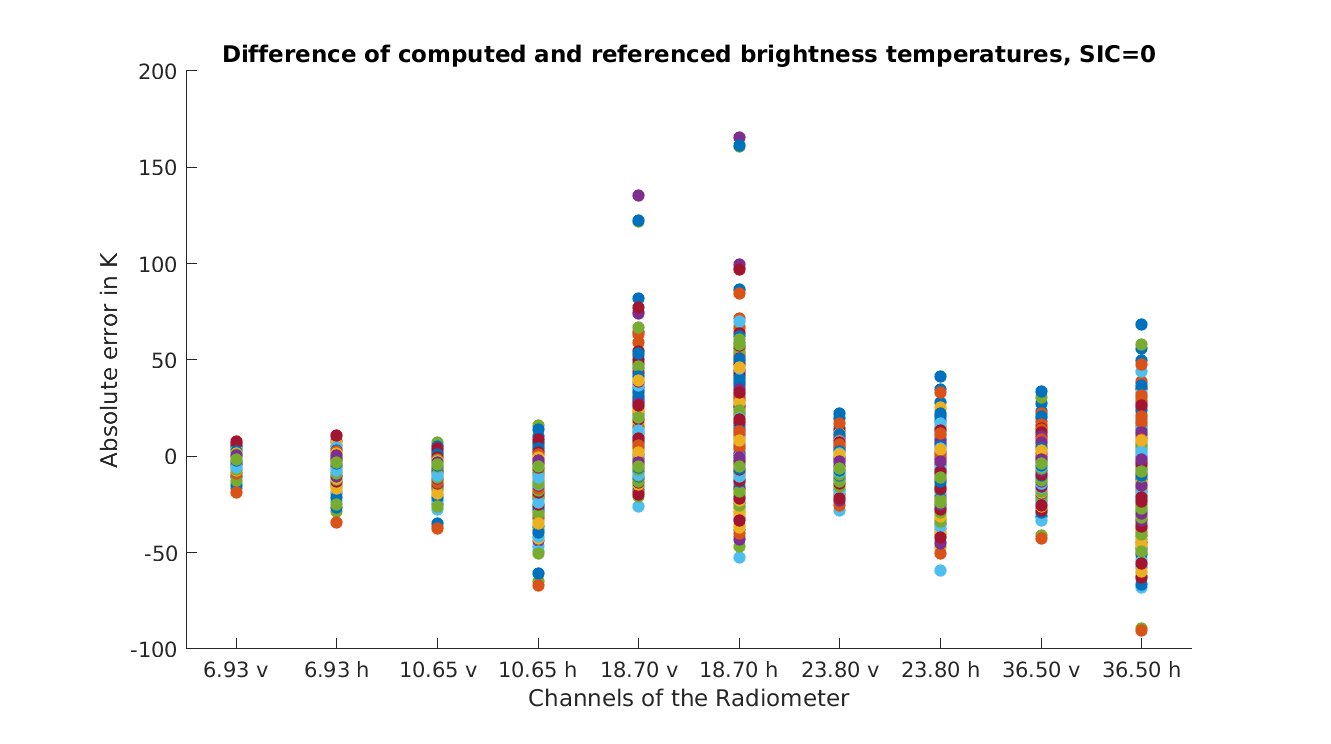
\includegraphics[width=0.9\textwidth]{ValidationForward_SIC0.eps}
   \caption{meaningful and informative caption}
   \label{fig:for0}
\end{figure}

\begin{figure}[h]
   \centering
   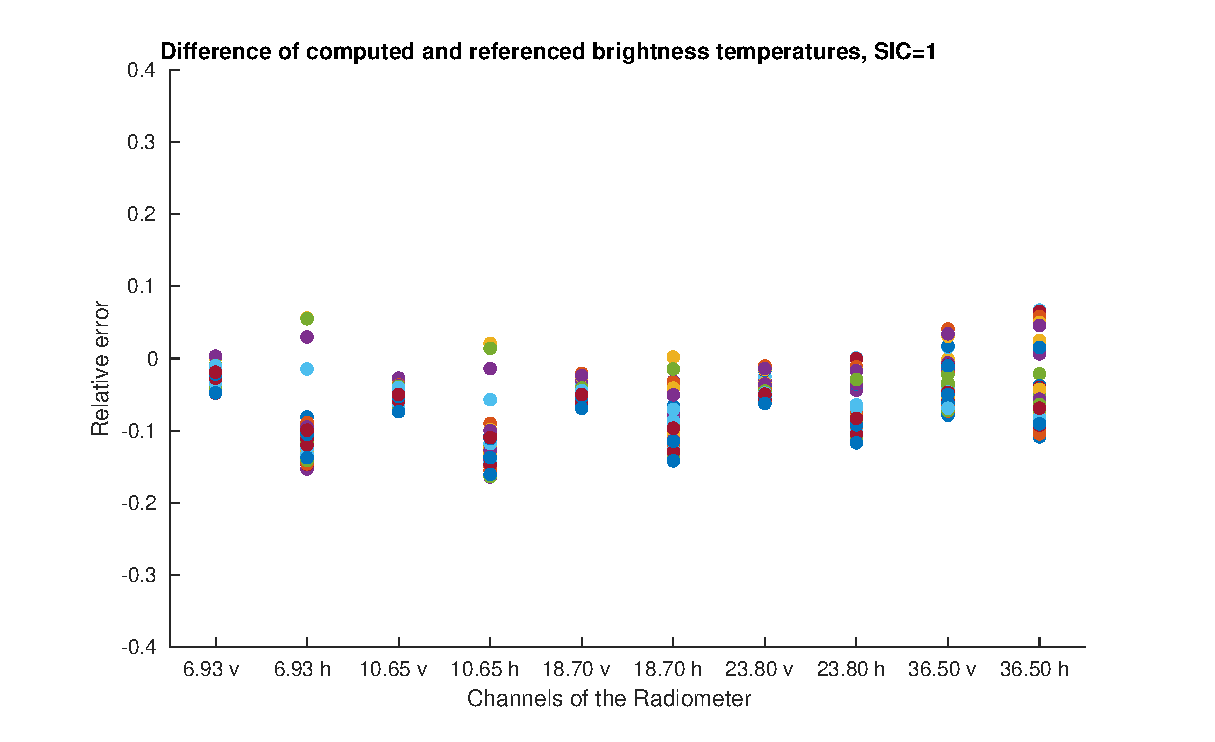
\includegraphics[width=0.9\textwidth]{ValidationForward_SIC1.eps}
   \caption{very relevant caption}
   \label{fig:for1}
\end{figure}

% Advanced Microwave Scanning Radiometer (AMSR) 
%The AMSR-E instrument on the NASA satellite EOS Aqua was operational between May 4, 2002 and October 4, 2011, and the AMSR2 instrument mounted on the JAXA satellite GCOM-W1, has been in operation since May 18, 2012. 

Firstly, the forward model was developed for the AMSR-E instrument. By using the numerical wheather predictions as input in the forward model in order to compare the output with the AMSR2 measured brightness temperatures, we assume that any calibration differences between AMSR-E and AMSR2 are negligible. 
\newline

Secondly, the reference data does not contain information about all geophysical paramters needed as input in the forward model. The multi-year ice fraction cannot be found in the reference data and should therefore be determined by other means. The reference data is divided into two parts, one contains only datapoints from areas of open water for which the ice concentration is zero in which case the MY fraction is also zero. It is therefore possible to test the forward model for the open water datapoints. The other part of the reference data contain datapoints from areas of high ice concentration for which the MY fraction is unknown. We will still attempt to test the forward model for the high ice concentration areas by making an estimate of the MY fraction through a process of trial and error. The idea is to select a location where we have prior information about the MY fraction(...).
\newline

Thirdly, the wind speed is given in the NWP reference data as a u-component, v-component, and as a composite of the two. (comment/question: where u and v denote zonal and meridional directions respectively?) We have used the composite value for the wind speed as the input in our forward model. (Argumentation!?) (-backscatter as a result of wind speed direction (upwind, downwind, crosswind) sensitive to azimuth angle \cite{Elachi})
\newline

In order to use the reference data in the forward model it was necesarry to perform unit conversions for the parameters water vapour and cloud liquid water, which were given in the columnar units of $\SI{1}{kg/m^2}$ in the reference data, and have now been converted to $\SI{1}{mm}$, indicating the height of water vapor or cloud liquid water if condensed uniformly across the column \cite{remss}. \newline


%\begin{itemize}
%\item \SI{1}{mm} equals \SI{1}{kg/m^2}
%\item calibration differences mentioned in Leif's email
%\item wind direction (several components given in the reference data)
%\item ice temperature layers (several given in the reference data)
%\item MY ice fractions not being given in the reference data
%\end{itemize}

% the assumption that "mm columnar" is equal to "kg/m2" is taken from here: http://www.remss.com/measurements/atmospheric-water-vapor/






\begin{thebibliography}{99}
	\bibitem[1]{Dorthe} Dorthe Hofman-Bang, Forward algorithm, September 2003. \newline \url{http://www.seaice.dk/exercises/task3/Matlab/FW_funktion2_is.m} \newline [accessed: 18/11/2017]
	
	%\bibitem[]{IOMASAreport} Dorthe Hofman-Bang and Leif Toudal, Estimating Ice, Ocean and Atmospheric Parameters from Polar Regions from AMSR-E Microwave Radiometer Measurements, Danish Center for Remote Sensing, Technical University of Denmark. 
	
	\bibitem[2]{Wink2} Round Robin Data Package Manual, Version 2.0/, July 2017. Ref: SICCI SIC RRDP-07-17. \newline
	\url{http://www.seaice.dk/undervisning/Sotiris/SICCI_RRDB_Manual_v2.01_20170717.docx} [accessed: 18/11/2017]
	
	\bibitem[3]{remss} (unit conversion) \url{http://www.remss.com/measurements/atmospheric-water-vapor/} [accessed: 18/11/2017]
	
	\bibitem[4]{Elachi}  C. Elachi, Introduction to the Physics and Techniques of Remote Sensing. John Wiley and Sons, 1987. (section 6.5+7.3)
	%(Hennings reference in his radar altimetry slides for wind speed direction discussion)
	
\end{thebibliography}

\end{document}






